%%%%%%%%%%%%%%%%%%%%%%%%%%%%%%%%%%%%%%%%%%%%%%%%%%%%%%%%%%%%%%%%%%%%%%%%%%%%%%%%%%%%%%%%%
% Appendix D: RapidSmith Checkpoints 
%	This section provides a overview of the contents of a RapidSmith Checkpoint
%   (RSCP). A very detailed description of TCPs is given in Thomas Townsend's 
%   Masters thesis available at http://scholarsarchive.byu.edu/etd/6492/
%%%%%%%%%%%%%%%%%%%%%%%%%%%%%%%%%%%%%%%%%%%%%%%%%%%%%%%%%%%%%%%%%%%%%%%%%%%%%%%%%%%%%%%%%
\newpage
\section{VDI Checkpoint Formats} \label{sec:rscpTcp}
\graphicspath{{./techReportFigures/appendixD/} {./techReportFigures/sec5_designs/}}

Before reading this appendix, it is encouraged for the reader to first read
Thomas Townsend's master thesis located for download at: {\color{blue}
http://scholarsarchive.byu.edu/etd/6492/}. This document gives a very detailed
introduction to the \textbf{Vivado Design Interface}, the interface used to
extract device and design information out of Vivado. 

\vspace{.3cm}

Vivado Tcl commands are used to define an alternate checkpoint representation
for open-source tools. VDI defines two different external design
representations:

\begin{enumerate}
  \item \textbf{RapidSmith Checkpoints (RSCP)}: Represents designs that have
  just been exported from Vivado. These checkpoints are intended to be loaded
  into external tools.
  \item \textbf{Tincr Checkpoints (TCP)}: Represents designs
  that can be loaded back into Vivado.
\end{enumerate}

\noindent Each of these checkpoints are capable of representing a Vivado design
post-synthesis, post-place, and post-route, enabling the design flows shown 
\autoref{fig:vdiDesign}. The remainder of this chapter describes each external
design representation, and the required Tcl commands to generate each.
Section \ref{sec:vdiImport} introduces RSCPs and Section~\ref{sec:vdiExport} introduces
TCPs. Section \ref{sec:tclChallenges} lists the variety of Tcl challenges
associated with using the Vivado Tcl interface to represent designs externally.
Section \ref{sec:twoFormats} includes a discussion on why two different external
design formats are necessary. The purpose of this appendix is to document the
format of RSCPs and TCPs so that maintainers of RapidSmith2 will understand how
to parse/generate these files. These checkpoint formats may change with future
versions of Vivado. \textbf{General users of RapidSmith2 can ignore this
appendix}.

\begin{figure}[h!]
  \centering
  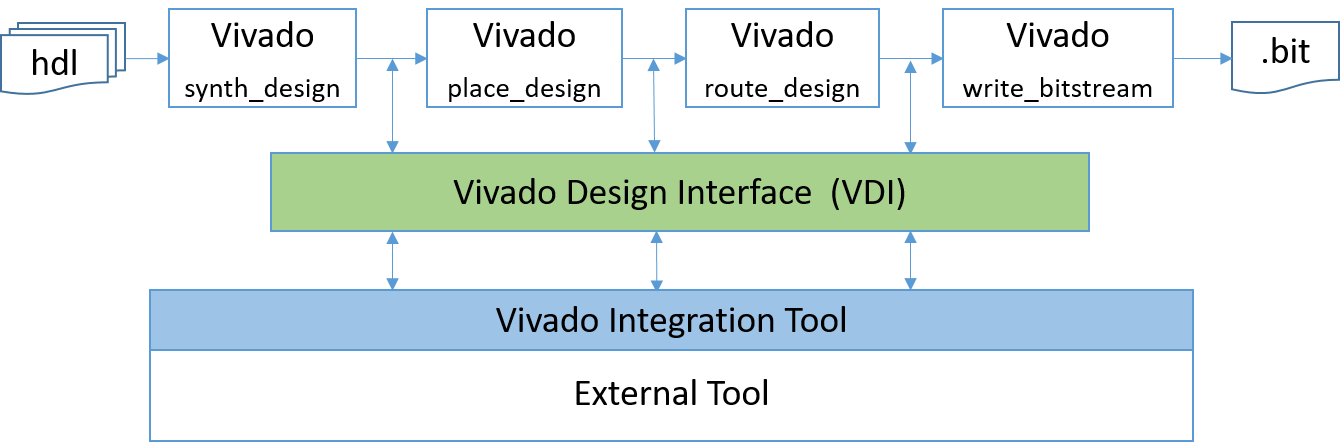
\includegraphics[width=.9\columnwidth]{vdiDesign.png}
  \caption{Vivado Design Interface (VDI) Design Flows}
  \label{fig:vdiDesign}
\end{figure}

%%%%%%%%%%%%%%%%%%%%%%%%%%%%%%%%%%%%%
%			RSCPs
%%%%%%%%%%%%%%%%%%%%%%%%%%%%%%%%%%%%%
\subsection{Design Export (RSCP Format)} \label{sec:vdiImport}
% TODO: mention that an RSCP can represent a Vivado design post synth, place or
% route.
VDI exports Vivado FPGA designs in the form of \textbf{RapidSmith Checkpoints}
(RSCP). A RSCP is a fileset containing 6 individual files: 

% Have a individual section for each of these and then discuss the Vivado Tcl
% challenged individually
\begin{multicols}{2}
	\begin {itemize}
	  \item design.info
	  \item netlist.edf
	  \item macros.xml
	  \item contraints.xdc
	  \item placement.rsc
	  \item routing.rsc
	\end{itemize}
\end{multicols}

\noindent Each file represents a specific aspect of a Vivado FPGA design, and
is described in the following subsections. The new \texttt{Tincr} command
\texttt{[tincr::write\_rscp]} can generate valid RSCPs for
\textbf{fully-flattened} Vivado designs. It is important to note that the name
``RapidSmith'' does not make the checkpoints exclusive to RapidSmith. The name
was arbitrarily chosen to match the external CAD framework used to test and
validate VDI. Any external tool that desires to operate on Vivado designs can
use these checkpoints.

\subsubsection{Design.info}
The \textit{design.info} file of a RSCP is reserved for additional information
about a design that is not related to the design netlist or implementation. It
currently only holds two pieces of information: (1) the part name that the
design is implemented on, and (2) the checkpoint ``mode''. The part name is
technically redundant, in that it is also included in the EDIF netlist
(described in the next subsection), but can be easier to parse than its EDIF equivalent. The
checkpoint mode refers to the type of checkpoint that was exported from Vivado.
If the Vivado design was implemented out-of-context, then the mode value will
be \texttt{out\_of\_context}. Otherwise, the mode value will be
\texttt{regular}. Because out-of-context checkpoints do not route to
peripheral FPGA pins, external tools or frameworks that parse RSCPs may need to
handle out-of-context designs differently. \autoref{lst:designInfo} shows an
example \textit{design.info} file. 

\begin{lstlisting}[numbers=none, keywordstyle=, stringstyle=, caption=
Sample design.info, label=lst:designInfo]
  part=xc7a100tcsg324-3
  mode=out_of_context	
\end{lstlisting}

\subsubsection{Netlist.edf}
The \textit{netlist.edf} file within a RSCP is an EDIF netlist representing the
logical portion of a design. It details all cells, nets, and
top-level ports within a design, and is generated from Vivado using the Tcl
command \texttt{[write\_edif]}. An example EDIF file is shown
\autoref{lst:edif}. External tools can use any open-source EDIF parser (such as
BYU EDIF tools) to translate the EDIF into their own design representation to
perform netlist modifications.

\begin{lstlisting}[numbers=none, keywordstyle=, stringstyle=, caption=
Sample EDIF, label=lst:edif]
  (Library work
    (edifLevel 0)
    (technology (numberDefinition ))
    (cell add (celltype GENERIC)
      (view add (viewtype NETLIST)
        (interface
          (port a (direction INPUT))
          (port b (direction INPUT))
          ...
        )
        (contents
          (instance cout_OBUF (viewref netlist (cellref OBUF (lib hdi_primitives))))
          (instance cout_lUT (viewref netlist (cellref LUT3 (libref hdi_primitives))) 
            (property INIT (string "8'hE8"))
          )
          ...	
\end{lstlisting}

\subsubsection{Constraints.xdc}
The \textit{constraints.xdc} file within a RSCP stores all user-defined XDC
constraints on a Vivado design. XDC constraint files are similar to UCF files
for ISE designs. Constraints can be used to set the clock frequency, constrain
a top-level port to a specific package pin on the device, and set other
physical implementation details. An example RSCP constraints file can be
seen in \autoref{lst:constraintsRsc}, and is essentially a list of Tcl commands.

\begin{lstlisting}[numbers=none, keywordstyle=, stringstyle=, caption=
Sample constraints.xdc, label=lst:constraintsRsc]
  create_clock -period 5.000 -name sysClk -waveform {0.000 2.500}
  set_property IOSTANDARD LVCMOS18 [get_ports clk]
  set_property IOSTANDARD LVCMOS18 [get_ports ena]
  set_property PACKAGE_PIN E15 [get_ports {Yin[12]}]
  set_property PACKAGE_PIN H17 [get_ports {Xin[14]}]
  set_property PACKAGE_PIN D18 [get_ports {Xin[7]}]
\end{lstlisting}

\subsubsection{Macros.xml} \label{sec:macrosRscp}

%  that had been flattened during synthesis
Many fully-flattened Vivado designs contain \textbf{hidden macros}. Hidden
macros are Vivado macro primitives that are not returned from the Tcl command
\texttt{[get\_lib\_cells]}, but are used in a netlist anyway. For example, the
macro primitive IOBUF is found in a variety of Series7 designs, but
the Vivado Tcl command \texttt{[get\_lib\_cells IOBUF]} returns an empty string
indicating that the library cell cannot be found. This breaks the well defined
assumption that \texttt{[get\_lib\_cells]} returns a list of \textit{all}
Xilinx primitives that can be used in a design netlist. Hidden macros create two
problems in particular:

\begin{enumerate}
  \item Because \texttt{[get\_lib\_cells]} is used to generate the cell library
   XML, the default cell library XML returned from
   \texttt{[tincr::create\_xml\_cell\_library]} is incomplete and only supports
   the subset of designs without hidden macros.
   \item Hidden macros are ``primitive" cells in Vivado's perspective.
   Therefore, the internal structure of hidden macros is not expanded in the
   \textit{netlist.edf} file described above. They are simply black box cells to
   external tools
\end{enumerate}

RSCPs handle hidden macros by including a \textit{macros.xml} file
which contains template information about each hidden macro in a Vivado design.
This file has the same format as regular cell library macros as shown in
\autoref{lst:macroXml}. External tools can augment their default cell library with
the cells found in \textit{macros.xml} to create a complete list of
primitives used in a given design. An alternative approach is to include
placement information for the macro. 

%VDI does not currently support relatively placed macros (RPM), making
%it difficult to fully represent Vivado designs using only a cell library and
%EDIF netlist. 

\subsubsection{Placement.rsc}

% TODO: add information about internal properties here

The \textit{placement.rsc} file within a RSCP stores all the placement
information of a Vivado design. Specifically, the file includes four different
tokens to differentiate placement data:

\begin{itemize}
  \item \textbf{LOC}: Gives the site and BEL that a cell in the
  netlist is placed on. An example is shown on line 3 of
  \autoref{lst:placementRsc}. In this case, the cell named
  ``cout\_OBUF\_inst\_i\_1'' is placed onto the ``A6LUT'' BEL of the
  ``SLICE\_X0Y51'' site. The site type (SLICEL) is also given after the site
  name in case the site needs to be changed to an alternate type before
  placing the cell (not required for the example cell placement). 
  
  \item \textbf{PINMAP}: Gives the logical-to-physical mapping for each cell
  pin attached to a given cell. Line 4 of \autoref{lst:placementRsc} shows the
  cell pin mappings for ``cout\_OBUF\_inst\_i\_1.'' As can be seen, the
  ``O'' cell pin is mapped to the ``O6'' BEL pin of the A6LUT, the I0 cell pin
  is mapped to the A4 BEL pin, etc. These pin mappings are required in
  \textit{placement.rsc} because certain cells can have different pin mappings
  based on how they are configured.  For example, the pin mappings for a BRAM
  cell with a data width of 72 bits differ from the pin mappings of the same
  BRAM cell with a data width of 9 bits, even if they are placed at the same
  physical location. \texttt{PINMAP} tokens help external tools guarantee
  that the pin mappings for each cell are correct. Cell pin mappings
  contained in the cell library are for the cell's \textbf{default
  configuration} only. Future work includes creating a more detailed pin
  mapping in the cell library so that the \texttt{PINMAP} token is no longer
  required in \textit{placement.rsc}.
  
  \item \textbf{PACKAGE\_PIN}: Gives the site and BEL that a top-level port
  is mapped to. Line 6 of \autoref{lst:placementRsc} shows an example for a port
  named ``fsync\_out.'' In this case, ``fsync\_out'' is mapped to the ``PAD'' BEL on
  the ``IOB\_X1Y30'' site.
  
  \item \textbf{IPROP}: Gives the value of an internal cell property (to a
  macro). Internal cell properties are not included within in the EDIF
  netlist, and so are included in \textit{placement.rsc} for completeness. 
\end{itemize}

\noindent If a design has not yet been placed, \textit{placement.rsc} will be
empty. It is important to note that for macro primitives in a design, only the
placement information for internal cells to the macro are included.
\autoref{lst:placementRsc} demonstrates the order in which the above tokens
appear in the file. \autoref{fig:cellPlacement} shows a visual representation
of how cells are placed onto BELs in Vivado.

\begin{lstlisting}[xleftmargin=1.5em, framexleftmargin=1.5em, keywordstyle=,
stringstyle=, caption= Sample placement.rsc, label=lst:placementRsc]
	IPROP seq_ram_reg_0_127_0_0/DP.HIGH INIT 64'h0000000000000000
	...
	LOC a_IBUF_inst R10 IOB33 INBUF_EN
	PINMAP a_IBUF_inst O:OUT I:PAD
	LOC cout_OBUF_inst_i_1 SLICE_X0Y51 SLICEL A6LUT
	PINMAP cout_OBUF_inst_i_1 O:O6 I0:A4 I1:A5 I2:A6
	...
	PACKAGE_PIN fsync_out IOB_X1Y30 PAD
	PACKAGE_PIN data_out[7] IOB_X1Y33 PAD
	...  
\end{lstlisting}

\begin{figure}[h!]
  \centering
  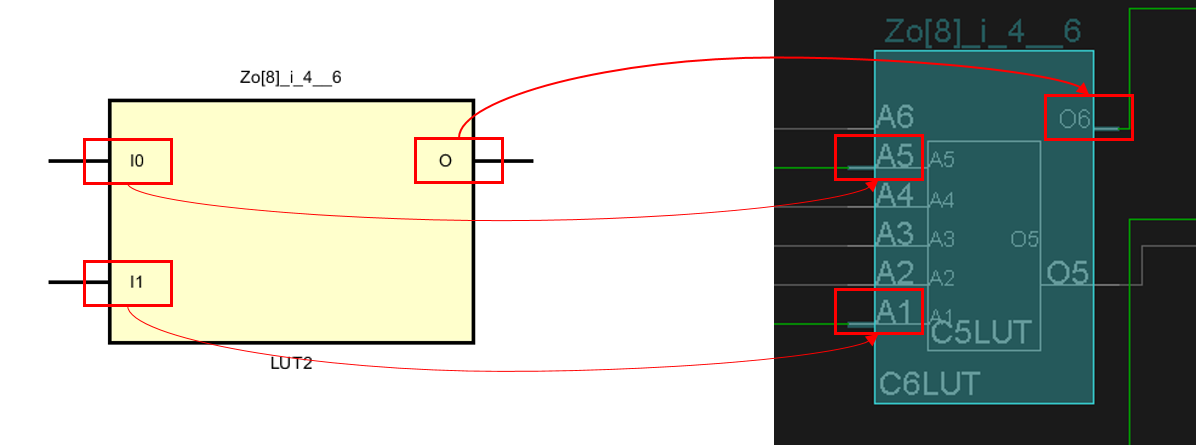
\includegraphics[width=\columnwidth]{cellPlacement.png}
  \caption{Example Cell Placement}
  \label{fig:cellPlacement}
\end{figure}

\subsubsection{Routing.rsc} \label{sec:routingRsc}

The \textit{routing.rsc} file is the most complex file of a RSCP, and stores a
complete description of all routing resources used in a Vivado design.
Specifically, it contains the following:

\begin{itemize}
  \item The intrasite routing configuration for each site in the form of
  used site PIPs (routing muxes)
  \item A list of BELs configured as routethroughs (both LUT and flip-flops).
  %This includes the input pin, output pin, and BEL of each routethrough.
  \item A list of BELs configured as static VCC/GND sources. 
  \item \textbf{Intrasite} nets.
  \item Routed \textbf{intersite} nets with their corresponding site pins and
  used PIPs.
  \item The \textbf{merged} physical routing information for VCC and GND nets.
\end{itemize}


\noindent An example \textit{routing.rsc} is shown in \autoref{lst:routingRsc}.
If a design has not yet been routed, only the intrasite routing information will be
included in this file. If the design has not yet been placed, this file will be
empty. The rest of this section describes each component within a
\textit{routing.rsc} file, and how they can be determined in Vivado.

\begin{lstlisting}[xleftmargin=1.5em, framexleftmargin=1.5em, keywordstyle=,
stringstyle=, caption= Sample routing.rsc, label=lst:routingRsc]
	SITE_PIPS SLICE_X9Y80 SRUSEDMUX:0 CEUSEDMUX:IN CLKINV:CLK  ...
	SITE_PIPS SLICE_X13Y80 PRECYINIT:AX SRUSEDMUX:0 COUTUSED:0 ...
	...
	VCC_SOURCES SLICE_X5Y104/C6LUT/O6 SLICE_X5Y102/C6LUT/O6 ...
	GND_SOURCES SLICE_X2Y106/D6LUT/O6 SLICE_X2Y106/C6LUT/O6 ...
	LUT_RTS SLICE_X5Y101/B6LUT/A6/O6 SLICE_X40Y96/DFF/D/Q  ...
	...
	INTRASITE AddSub[10]
	INTERSITE AngStep1[0] SLICE_X2Y82/AX SLICE_X2Y87/AQ SLICE_X2Y84/A1 ... 
	ROUTE AngStep1[0] INT_X28Y26/INT.LOGIC_OUTS_W1->>SDNDSW_W_0_FTS ...
	...
	VCC INT_L_X2Y107/INT_L.VCC_WIRE->>IMUX_L42 ...
	START_WIRES INT_L_X2Y107/VCC_WIRE INT_L_X2Y106/VCC_WIRE ...
	GND INT_R_X3Y106/INT_R.GND_WIRE->>GFAN1 ...
	START_WIRES INT_R_X3Y106/GND_WIRE INT_L_X4Y106/GND_WIRE ...
\end{lstlisting}

\subsubsection{Site PIPs}

The internal routing structure of nets inside Vivado sites are represented by
a set of used site PIPs. A string of site PIPs enables a connection between site
components. An example is shown in \autoref{fig:sitePips2} where the used site
PIPs are circled in red. As can be seen, the \texttt{ACY0:05} site PIP is
enabled and connects the \texttt{05} pin of the \texttt{A5LUT} BEL to the
\texttt{DI0} pin of the \texttt{CARRY4} BEL. Site PIPs can also be used to 
connect site pins to BEL pins. The Vivado Tcl command \texttt{[get\_site\_pips -of \$site -filter
IS\_USED]} can be used to obtain a list of used site PIPs within a given site.
\texttt{[tincr::write\_rscp]} formats the site pips as shown on line 1 and 2 of
\autoref{lst:routingRsc}. External tools can use the \texttt{SITE\_PIPS} token
within a \textit{routing.rsc} file to reconstruct the internal routing of
each site.

\begin{figure}[h!]
  \centering
  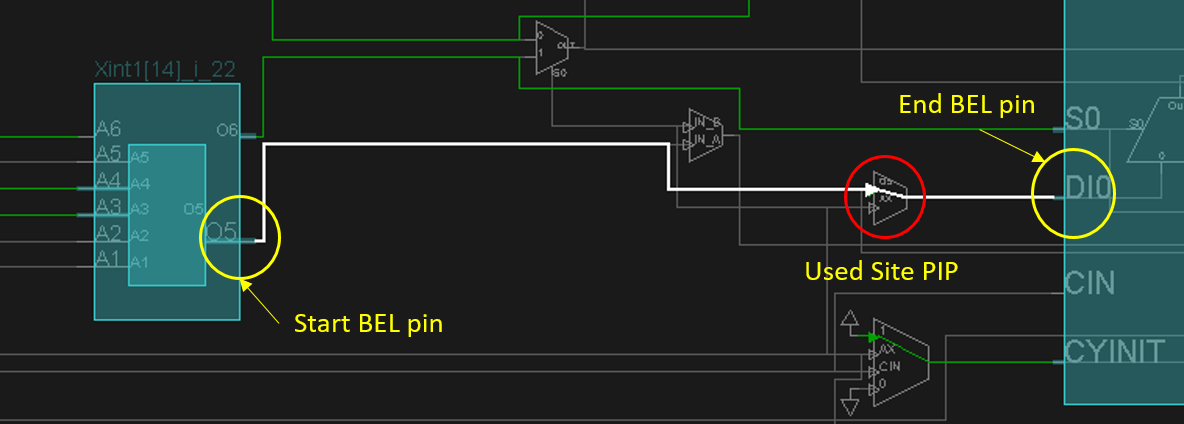
\includegraphics[width=\columnwidth]{sitePips.png}
  \caption{Site PIP Usage}
  \label{fig:sitePips2}
\end{figure}

\subsubsection{LUT Routethroughs} \label{sec:belRoutethroughs}
% TODO: explain here that no cell is placed on the bel?
Besides their use in implementing logic equations, LUT BELs can also be
configured as PIPs in a fully-routed FPGA design (known as a routethrough). A
LUT is marked as a routethrough when its configuration equation,
\texttt{CONFIG.EQN}, maps the value of a single input pin directly to the
output pin. For timing, the A6 pin is the most preferable option for
a routethrough since it is the fastest, but pins A1-A5 can also be
used in cases of routing congestion. Routethrough LUTs are not explicitly
represented in a design netlist since there is no cell placed on the
corresponding BEL, so they need to be included in the \textit{routing.rsc} of a
RSCP. Otherwise, designs could not be fully represented in external tools.
\autoref{fig:routethroughs2} shows two example routethrough LUTs in Vivado.

\begin{figure}[h]
  \centering
  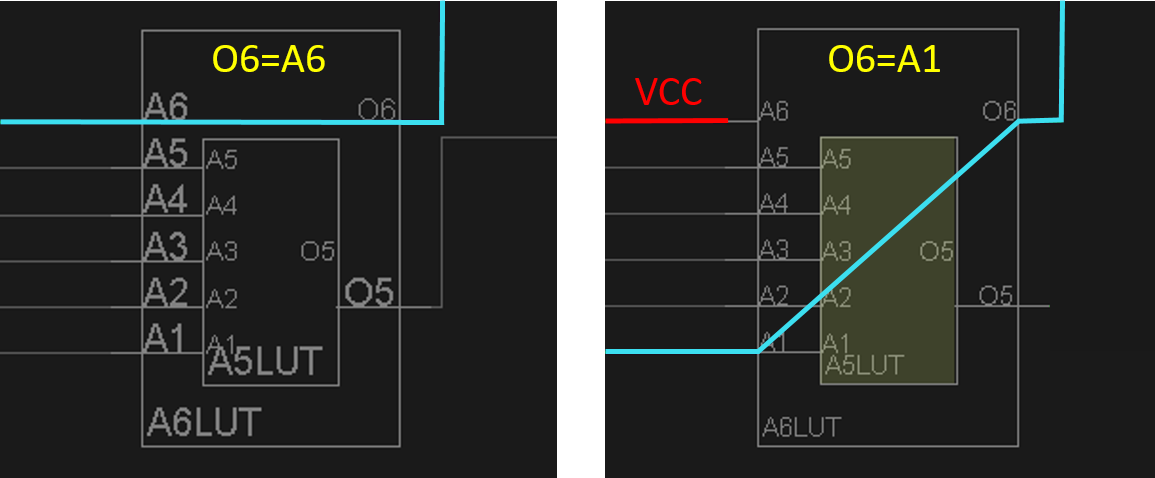
\includegraphics[width=5.5in]{routethroughs2.png}
  \caption{Two examples of LUTs configured as routethroughs in Vivado. The net
  highlighted in red represents VCC.}
  \label{fig:routethroughs2}
\end{figure}

For the LUT on the left, the input pin \texttt{A6} is mapped directly to the 
output pin \texttt{O6}. The corresponding configuration equation for this BEL is 
\texttt{CONFIG.EQN:O6=(A6)}. For the LUT on the right, the input pin \texttt{A1}
is mapped directly to the output pin \texttt{O6}. However, the structure of the
configuration equation for this LUT is slightly different. As 
\autoref{fig:routethroughs2} shows, VCC is routed to the \texttt{A6} input pin.
In this case, the configuration equation on the BEL is
\texttt{CONFIG.EQN:O6=(A6+{\textasciitilde}A6)*((A4))}. Using Vivado's TCL
interface, LUT routethroughs can be identified by matching their
\texttt{CONFIG.EQN} property against the Tcl regular expression

\begin{center}
\verb!(O[5,6])=(?:\(A6\+~A6\)\*)?\(+(A[1-6])\)+ ?!
.
\end{center}

On design export, LUTs that are identified as routethroughs are included
in the \textit{routing.rsc} file with the token \texttt{LUT\_RTS}. An example is
shown on line 6 of \autoref{lst:routingRsc}. Each routethrough is represented
in the form ``site/bel/input\_pin/output\_pin." It is important to note that not
all LUT BELs are tested for routethroughs. For an arbitrary LUT to be
used as a routethrough, it needs to satisfy three conditions. (1) Its parent
site needs to be used (i.e. there is at least one cell placed onto the site),
(2) no cell is currently placed on the corresponding bel, and (3) at least one
input bel pin is not currently being used.

\subsubsection{Permanent Latches}
A \textbf{permanent latch} in Vivado is a Flip Flop (FF) BEL which has been
configured as a latch with its ``set'' signal tied to VCC. This means that the
data pin of the latch always passes its value to the output pin of the latch,
and no state is retained. An example is shown in \autoref{fig:ffRoutethrough2}.
As the figure shows, permanent latches look very similar to LUT routethroughs
described in the previous section.

\begin{figure}[h]
  \centering
  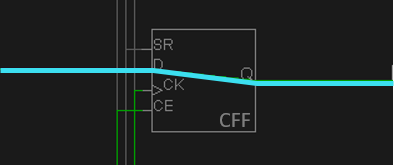
\includegraphics[width=.5\columnwidth]{ffRoutethrough.png}
  \caption{Flip-Flop BEL Configured as a Permanent Latch in Vivado}
  \label{fig:ffRoutethrough2}
\end{figure}

Because of this similarity, \textit{routing.rsc} files treat permanent latches
the same as LUT route-throughs. That is, each permanent latch is included
alongside the \texttt{LUT\_RTS} token as shown on line 6 of
\autoref{lst:routingRsc}. The string ``SLICE\_X40Y\-96/DFF/D/Q'' gives an
example of what a permanent latch looks like in the \textit{routing.rsc} file. Permanent
latches in Vivado can be identified based on two qualifications: (1) there is
no cell placed on the corresponding FF BEL, and (2) the property
\texttt{CONFIG.LATCH\_OR\_FF} of the BEL is set to \texttt{LATCH}.

\subsubsection{LUT Static Sources}
Similar to their use as routethroughs, LUT BELs can also be configured as GND or
VCC signal sources. Examples of both are shown in
\autoref{fig:lutStaticSources2}. The LUT on the left of the figure drives a VCC
signal and the LUT on the right drives GND. In both cases, the logical
netlist of a design does not represent the use of these LUTs in any way.
Therefore, the \textit{routing.rsc} file marks VCC and GND source LUTs with the
tokens \texttt{VCC\_SOURCES} and \texttt{GND\_SOURCES} respectively. This is
shown on line 4 and 5 of \autoref{lst:routingRsc}. External tools can use the
BELs marked \texttt{VCC\_SOURCES} and \texttt{GND\_SOURCES} to fully
recreate the routing of GND and VCC nets. Static source LUTs are identified
in Vivado by matching their \texttt{CONFIG.EQN} property against the Tcl regular
expression

\begin{center}
\verb!(O[5,6])=(?:\(A6\+~A6\)\*)?\(?[0,1]\)? ?!
.
\end{center}

\noindent LUTs that match the expression are formatted in
\textit{routing.rsc} with the form ``site/bel/source\_pin.'' It is important to
note that external CAD tools can also make use of this routing structure while
creating routing algorithms for Xilinx devices.

\begin{figure}[t]
  \centering
  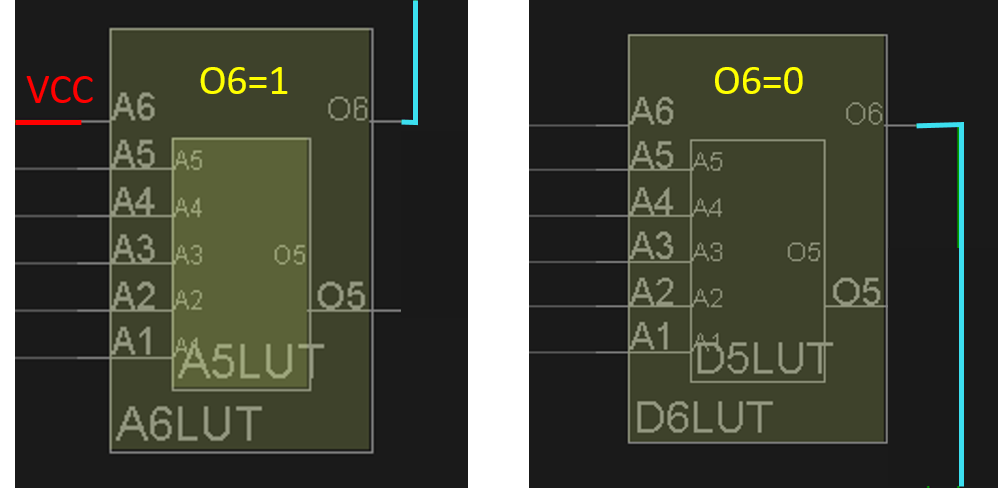
\includegraphics[width=.7\columnwidth]{lutStaticSources.png}
  \caption{Two LUTs Configured as Static Sources in Vivado}
  \label{fig:lutStaticSources2}
\end{figure}

\subsubsection{Intrasite Nets}

There are two types of nets in Vivado: \textbf{intrasite} nets and
\textbf{intersite} nets. Intrasite nets are those that are contained completely
within site boundaries. \autoref{fig:intrasite} shows an example intrasite net,
which connects to only BEL pins. The \textit{routing.rsc} file marks all
intrasite nets with the token \texttt{INTRASITE} as shown on line 8 of
\autoref{lst:routingRsc}. No additional information is given about
intrasite nets. External tools can reconstruct intrasite nets by using the
source BEL pin of the net in conjunction  with the used site pips of the
corresponding site. A list of intrasite nets can be obtained in Vivado with
the Tcl command \texttt{[get\_nets -filter \{ROUTE\_STATUS==INTRASITE\}]}.

\begin{figure}[b!]
  \centering
  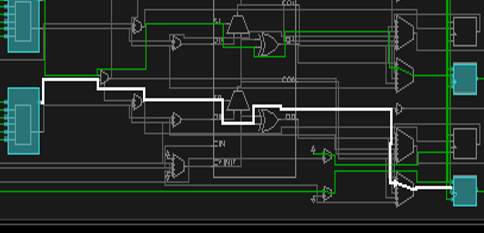
\includegraphics[width=.9\columnwidth, height=2in]{intrasite.png}
  \caption{Vivado Intrasite Net (highlighted in white)}
  \label{fig:intrasite}
\end{figure}

\subsubsection{Intersite Nets}

%Intersite nets have two different structures based on the current stage of
% design implementation.
A majority of nets in a FPGA design are \textbf{intersite} nets. Intersite nets
are those that use general routing fabric to connect cells across site
boundaries as shown in \autoref{fig:intersiteNet}.  After
a design has been placed in Vivado, each intersite net is partially routed.
That is, the intrasite portions of the net (the wires within sites) are routed
to site pins via site wires. To represent an intersite net at the placement
stage of implementation, the \textit{routing.rsc} file includes an
\texttt{INTERSITE} token, which lists all site pins a net is connected to. Line
9 of \autoref{lst:routingRsc} shows an example \texttt{INTERSITE}
specification. Site pins are important for recreating the routing structure of
nets in external tools because they can be used to (a) build the intrasite
portions of a net and (b) determine if a net is fully routed (nets that route
to all their site pins are fully routed by definition). In Vivado, the site pins
attached to a net can be determined with the Tcl command
\texttt{[get\_site\_pins -of \$net]}.

During the routing stage of implementation, all site pins of a net are connected
together through the general routing fabric of the FPGA. At this point the net
is considered fully routed. The physical structure of a fully routed net
can be expressed three different ways in Vivado:  (1) the ROUTE property on the
net, (2) the wires used in the net, or (3) the device PIPs used in the net. For
reasons discussed in Section~\ref{sec:tclChallenges}, device PIPs are the best option
for external tools. The \textit{routing.rsc} file uses the token \texttt{ROUTE}
for specifying the PIPs of a routed net. Line 10 of \autoref{lst:routingRsc}
shows an example \texttt{ROUTE} specification. The Tcl command
\texttt{[get\_pips -of \$net]} can be used to get a list of all PIPs being used
in a Vivado net. The RapidSmith2 import code contains an algorithm to convert
the pip list to a tree structure.

\begin{figure}[t!]
  \centering
  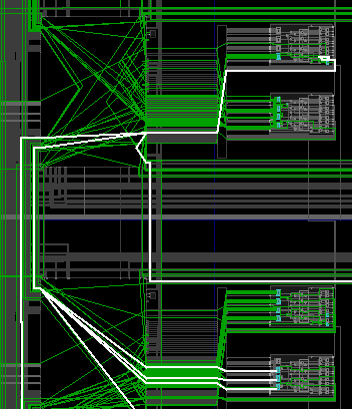
\includegraphics[width=.4\columnwidth]{intersiteNet.png}
  \caption{Vivado Intersite Net (highlighted in white)}
  \label{fig:intersiteNet}
\end{figure}

\subsubsection{VCC and GND Nets}

In general, a design can have more than one VCC net in the logical netlist. Each
of these nets should have their own unique physical information once the
design is routed (based on which wires they use), but this is not the case with
Vivado. Instead, Vivado reports that they each use the same set of wires which
correspond to a combination of \textit{all} VCC nets. The same applies to GND
nets. There are two possible solutions to resolve this discrepancy. The first is
to merge all logical VCC (or GND) nets in the netlist into a single net, matching
the merged physical routing. The second is to partition the physical
information so that each logical net has unique physical properties. 

For simplicity, RSCPs choose to implement the first option. Lines 12-15 of
\autoref{lst:routingRsc} show how VCC and GND nets are represented in a
\textit{routing.rsc} file. The \texttt{VCC} and \texttt{GND} tokens serve the
same purpose as \texttt{ROUTE}, they contain the used PIPs for all VCC and GND
nets. The \texttt{START\_WIRES} token gives a list of all wires connected to
VCC and GND sources. Starting at the specified start wires, VCC and GND nets
can be reconstructed in external tools. The Tcl command \texttt{[get\_nets
-filter \{TYPE==POWER\}]} is used to find all VCC nets in a design, and
\texttt{[get\_nets -filter \{TYPE==GROUND\}]} is used to find all GND nets
in a design. The start wires for VCC and GND nets are found by parsing their
corresponding \texttt{ROUTE} property strings.

%%%%%%%%%%%%%%%%%%%%%%%%%%%%%%%%%%%%%%%%%%%%
%				TCPs
%%%%%%%%%%%%%%%%%%%%%%%%%%%%%%%%%%%%%%%%%%%%
\subsection{Design Import (TCP Format)} \label{sec:vdiExport}

RSCPs are only used to represent exported Vivado designs and cannot be directly
imported back into Vivado. They must first be converted to \textbf{Tincr
Checkpoints} (TCP) in an external tool or framework. TCPs are a fileset proposed
in the original \texttt{Tincr} distribution, and serve as an alternate
representation of Vivado designs which can be imported into Vivado through the
VDI interface. Each TCP contains the following four files:

\begin{multicols}{2}
	\begin{itemize}
	  \item netlist.edf
	  \item constraints.xdc
	  \item placement.xdc
	  \item routing.xdc
	\end{itemize}
\end{multicols}

\noindent As can be seen, TCPs are largely based on Vivado XDC files, which
allow a subset of Tcl commands to set constraints on a variety
of Vivado objects. For example, cells can be placed and nets can be routed with
XDC constraints. The XDC format is desirable for two reasons in particular: (1)
a single Vivado Tcl command \texttt{[read\_xdc]} can parse and apply XDC
constraint files and (2) \texttt{[read\_xdc]} is much faster than regular Tcl
scripts executing the same commands.

Each file in a TCP represents a specific aspect of a Vivado FPGA design, and is
described in the following subsections as a review for the reader. The
\textit{netlist.edf} and \textit{contraints.xdc} file will not be reviewed
because they are identical to their RSCP counterparts presented in
Section~\ref{sec:vdiImport}. The \texttt{Tincr} function used to parse TCPs,
\texttt{[tincr::read\_tcp]}, has been updated in a variety of ways to support
fully importing Vivado designs. These modifications, and the limitations of
XDC, are described more in Section~\ref{sec:tclChallenges}

\subsubsection{Placement.xdc}
\autoref{lst:placementXdc} shows an example \textit{placement.xdc} file within a
TCP. Lines 1-3 of the listing show how a cell is placed in Vivado using XDC
commands. As can be seen, the first command sets the \texttt{BEL} property on
the cell to the corresponding \texttt{SITE\_TYPE.BEL\_NAME}. The second command
sets the \texttt{LOC} property on the cell, which specifies the actual site
location. The ordering of these commands relative to one another is crucial,
because if the \texttt{LOC} property is set before the \texttt{BEL} property an
error will be thrown in Vivado. For cells of group \texttt{LUT}, \texttt{INV},
or \texttt{BUF} the cell pin to BEL pin mappings must be set manually by the user. 
This can be done by setting the \texttt{LOCK\_PINS} property on the cell as
shown on line 3, and is most often used for LUT cells. Line 4 of
\autoref{lst:placementXdc} shows how a top-level port is mapped  to a FPGA
package pin.

\begin{lstlisting}[xleftmargin=1.5em, framexleftmargin=1.5em, keywordstyle=,
stringstyle=, caption= Sample placement.xdc, label=lst:placementXdc]
	set_property BEL SLICEM.H6LUT [get_cells {u3/angle.Ao[16]_i_3}]
	set_property LOC SLICE_X50Y30 [get_cells {u3/angle.Ao[16]_i_3}]
	set_property LOCK_PINS { I0:A3 I1:A1 } [get_cells {u3/angle.Ao[16]_i_3}]
	...
	set_property PACKAGE_PIN AD10 [get_ports {Rout[16]}]
	...	
\end{lstlisting}

\subsubsection{Routing.xdc} \label{sec:routingXdc}
During placement, the intrasite routing structure of each site is automatically
configured in Vivado based on what cells are placed onto the corresponding site.
Therefore, the only necessary information in the \textit{routing.xdc} file is
the intersite routing specification for each net. Specifically, the physical
structure of a net is specified in Vivado by setting its \texttt{ROUTE} string
property (also called a directed routing string) as shown in \autoref{lst:routingXdc}.
A directed routing string represents the tree structure of a physical
route by using nested brackets (``\{'') to represent branching. As an example,
take the hypothetical route shown in \autoref{fig:routeString}. One valid
\texttt{ROUTE} string associated with this route is \texttt{\{ A B \{ D E \} C
\}}. Another possible \texttt{ROUTE} string is \texttt{\{ A B \{ C \} D E \}},
they both represent the route shown in the figure. \texttt{ROUTE} strings can be
formatted to either include the tile of each wire (line 2 of
\autoref{lst:routingXdc}), or use only relative wire names (line 3 of
\autoref{lst:routingXdc}). The advantage of including tile names is to remove
any possible ambiguity for a route. The advantage of using relative wire names
is that they result in smaller \textit{routing.xdc} files. It is considered
best practice, however, to format \texttt{ROUTE} strings using tile names
to ensure the correctness of the route when it is imported into Vivado. 

\begin{lstlisting}[xleftmargin=1.5em, framexleftmargin=1.5em,keywordstyle=,
stringstyle=, caption= Sample routing.xdc, label=lst:routingXdc]
	...
	set_property ROUTE { CLEL_R_X36Y8/CLE_L_SITE_0_COUT ... }  [get_nets {Zo}]
	set_property ROUTE { CLE_L_SITE_0_COUT ... }  [get_nets {Zo}]
	...
\end{lstlisting}

\begin{figure}[t!]
  \centering
  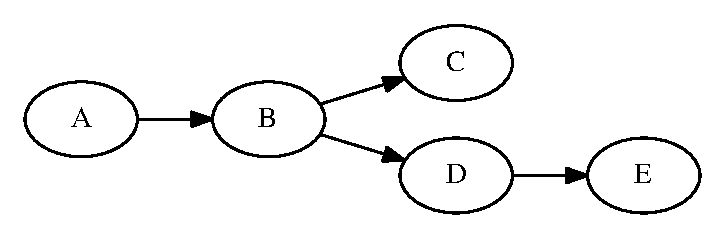
\includegraphics[width=.8\columnwidth]{routeString.eps}
  \caption{Sample Route (A, B, C, D, and E represent device wires)}
  \label{fig:routeString}
\end{figure}

%%%%%%%%%%%%%%%%%%%%%%%%%%%%%%%%%%%%%%%%%%%%
%		Tcl Interface Challenges
%%%%%%%%%%%%%%%%%%%%%%%%%%%%%%%%%%%%%%%%%%%%
\subsection{Vivado Tcl Interface Challenges} \label{sec:tclChallenges}

Vivado's Tcl interface supplies the necessary functionality to generate and
parse external design representations. VDI uses the interface to define the
formats for RSCPs and TCPs as described in the previous sections. There are,
however, a variety of challenges associated with using Tcl commands to generate
RSCPs and parse TCPs. Broadly, these challenges can be grouped into four
distinct categories.

\begin{enumerate}
  \item Vivado design import rules: External designs need to be imported
  into Vivado in a very specific way, or else import can fail. 
  \item Logical to physical mismatches: When a netlist is implemented on a
  device, most physical components match to a corresponding logical component
  (i.e. a BEL maps to a cell). But, there are some aspects of an
  implemented design that aren't represented in the logical netlist.
  \item Tcl objects that are incomplete, ambiguous, or return incorrect
  results when queried.
  \item Parts of a device or design that cannot be configured with Tcl commands
\end{enumerate}

\noindent The following subsections document each issue associated with
generating RSCPs or parsing TCPs, with their appropriate workaround. In some
cases, it is up to external tools to provide a solution. As previously
mentioned, each of these issues is specific to Vivado 2016.2, and may be fixed
in future tool versions.

%and help give a better understanding of why
%two different external design representations are necessary. 

\subsubsection{Ambiguous ROUTE Strings} \label{sec:routeStrings}

As described in Section~\ref{sec:routingXdc}, the \texttt{ROUTE} property
on a net contains its physical routing structure. By default, Vivado uses
relative wire names (no tile information) when building these \texttt{ROUTE}
strings. This is problematic for external tools because it can lead to wire
ambiguities. Specifically, it is possible for a given wire in a Xilinx FPGA
to connect to more than one wire of the same name. The 
\texttt{BRAM\_L\_X6Y170/BRAM\_CASCOUT\_ADDRBWRADDRU6} wire in the Artix7 part
\texttt{xc7a100tcsg324-3} is an example. This wire connects to two different
wires named \texttt{BRAM\_ADDRBWRADDRU6} through PIP connections.
The first wire is located in tile \texttt{BRAM\_L\_X6Y165} and the second wire
is located in tile \texttt{BRAM\_L\_X6Y175}. \autoref{lst:ambigRoute} shows how
Vivado distinguishes these two connections within \texttt{ROUTE} strings.

\begin{lstlisting}[xleftmargin=1.5em, framexleftmargin=1.5em, keywordstyle=,
stringstyle=, caption= Ambiguous ROUTE string example, label=lst:ambigRoute, escapeinside=||]
	// Tile  BRAM_L_X6Y165
	{ ...  BRAM_CASCOUT_ADDRBWRADDRU6 BRAM_ADDRBWRADDRU6  ... }
	// Tile BRAM_L_X6Y175 
	{ ...  BRAM_CASCOUT_ADDRBWRADDRU6 |\textbf{<1>}|BRAM_ADDRBWRADDRU6  ... }
\end{lstlisting}

\noindent As can be seen, the token ``\textless1\textgreater" is used to
differentiate the two wires. Vivado most likely has an internal data
structure that uses the token to choose the correct sink wire.  External
tools, however, don't have access to this data structure, meaning the only
option is to guess which wire is actually taken (clearly not an acceptable
solution). Ambiguous \texttt{ROUTE} strings are the primary reason why RSCPs use
PIPs to represent routing, and two different external formats are required.
 
\subsubsection{Alternate Site Pins}

As discussed in Section~\ref{sec:alternateSites}, the Vivado Tcl command
\texttt{[get\_site\_pins -of \$site]} does not return the correct result for
alternate sites on Series7 devices\footnote{UltraScale devices always return
the correct result}. An example of this behavior is shown in
\autoref{fig:alternateSitePins}. The site pin names clearly change in the GUI
after the site is changed to be of type \texttt{RAMB18E1}, but the Tcl
interface is not updated accordingly. RSCPs depend on exporting a correct set
of site pins for each net, but the reported site pins will be incorrect for
alternate sites if the above command is used.

\begin{figure}[h!]
  \centering
  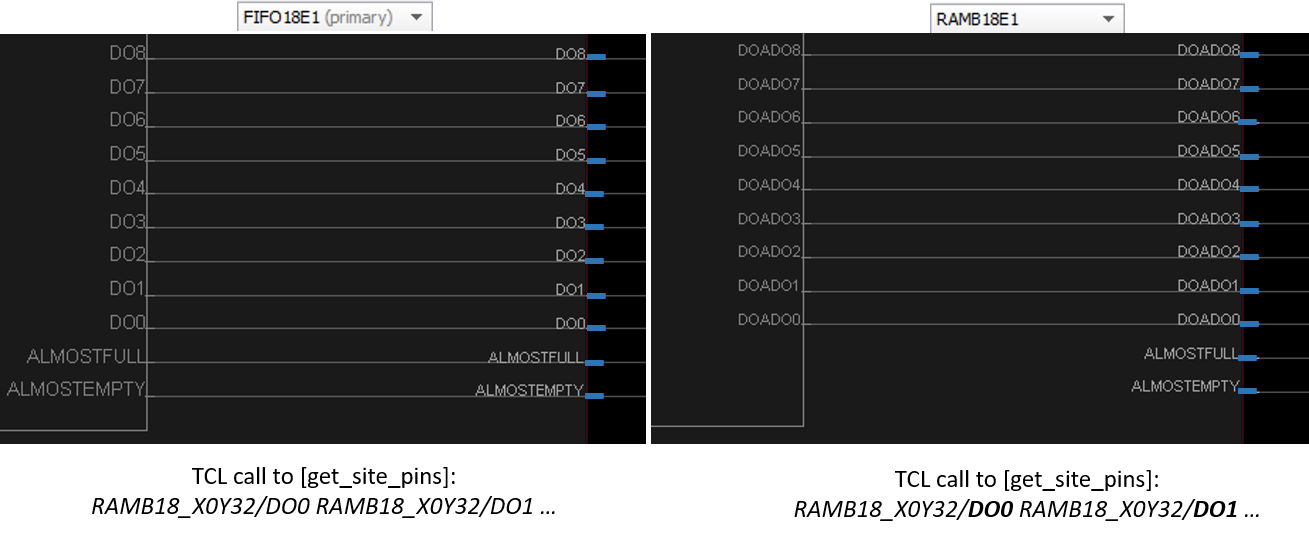
\includegraphics[width=\columnwidth]{alternateSitePins.png}
  \caption{An example of [get\_site\_pins] returning incorrect results in
  Vivado}
  \label{fig:alternateSitePins}
\end{figure}

VDI fixes this issue with an assumption about single-BEL sites in Series7
devices. As can be seen in \autoref{fig:alternateSitePins}, each BEL pin within
a single-BEL site connects to an identically named site pin. Using this
assumption and a customized site pin getter, the VDI command
\texttt{[tincr::write\_rscp]} reports the correct site pins for each net
connected to an alternate site. Of course, this is only valid if all alternate
types with changing site pins have a single BEL. Through experimentation
with several different designs, this appears to be true. As more tests are run
on Series7 devices and designs, the conclusion will be further tested for
validity.

\subsubsection{VCC/GND BEL Pins} \label{sec:vccGndBelPins}
% TODO: see if we can determine this in Vivado by looking at a nets BEL pins.
Most nets in a Vivado design connect to a set of cell pins, and are routed to
the corresponding BEL pins of those cell pins. VCC and GND nets,
however, can route directly to BEL pins that don't have a connecting cell pin.
An example is shown in \autoref{fig:pseudoCellPin2}. As the figure shows, VCC is
routed to the \texttt{A6} pin of the \texttt{D6LUT}, but there is no cell pin
mapped to \texttt{A6} (the input pins of the cell placed at the LUT have
been mapped to \texttt{A1} and \texttt{A4}). The fact that VCC connects to the
\texttt{A6} pin of this LUT is not represented in the logical netlist, and is purely an
implementation detail of the design. Lacking this information is particularly
challenging when developing routing algorithms in external tools. How will the
algorithm know to route to VCC/GND BEL pins when they are not explicitly
represented in the netlist? Unfortunately, these BEL pins cannot currently be
determined with Vivado Tcl commands, and so are not included in RSCPs. It is up
to external tools to understand the placement configurations that require VCC
and GND to be routed to individual BEL pins.

\begin{figure}[t]
  \centering
  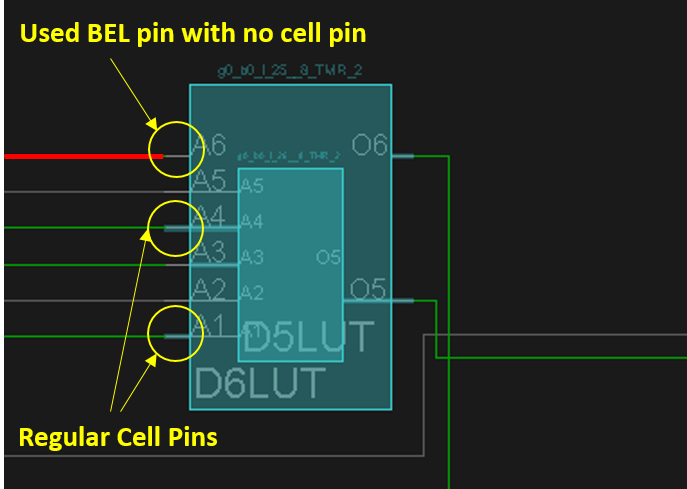
\includegraphics[width=.6\columnwidth]{pseudoCellPin.png}
  \caption{An example of VCC routing to an unused BEL pin (A6)}
  \label{fig:pseudoCellPin2}
\end{figure}

\subsubsection{SLICE Placement Order} \label{sec:slicePlacementOrder}

\begin{figure}[b!]
  \centering
  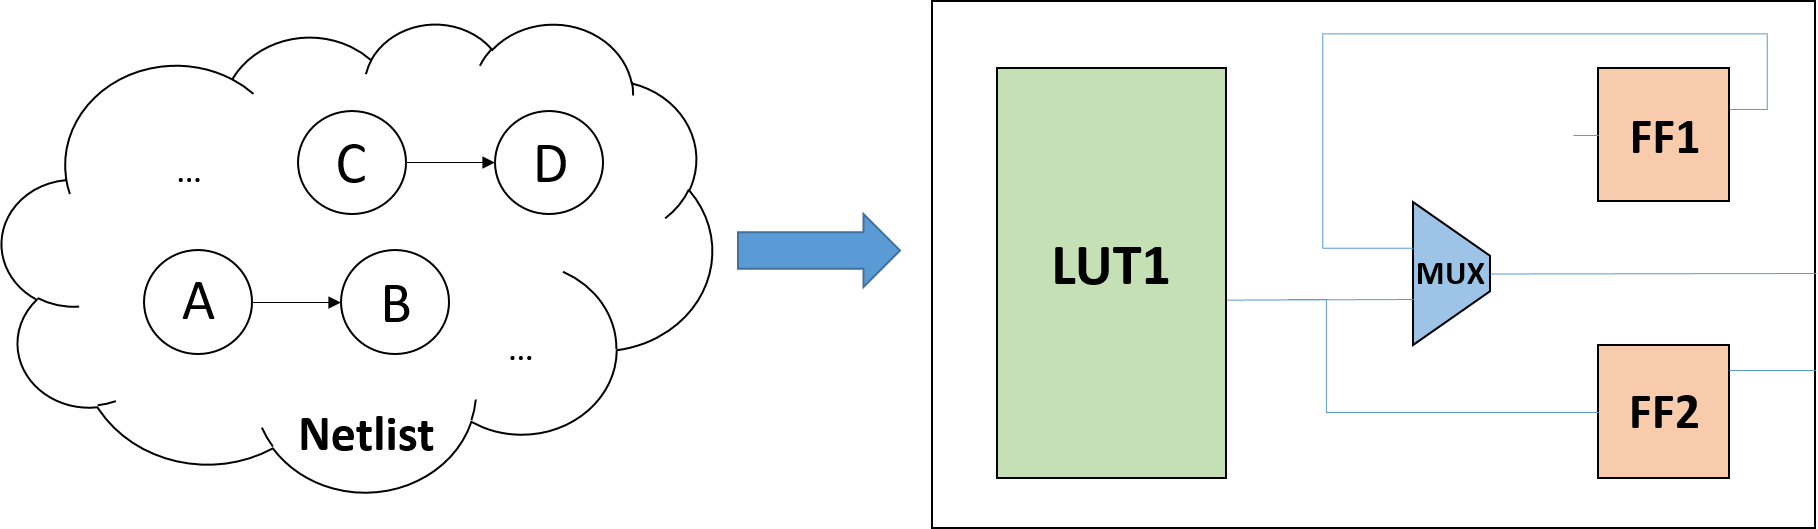
\includegraphics[width=\columnwidth]{contention.png}
  \caption{Routing Contention Example}
  \label{fig:contention}
\end{figure}

When a cell is placed in Vivado using Tcl API calls, Vivado
automatically configures the routing resources inside of the
corresponding site based on the cell's connections. Because
of this behavior it is possible to have a valid cell placement,
but to place the cells in an order that causes an illegal routing
configuration (i.e. a routing mux is optionally being used by
a net, but is required by a different net of a cell that has just
been placed). This primarily affects sites of type SLICEL
and SLICEM, due to their more complex internal routing. 

\autoref{fig:contention} shows a simplified example of why routing contention
can happen within SLICE sites. In this hypothetical scenario, the netlist in
the left of the figure is  placed onto the site in the right of the 
figure. Assume the cells of the netlist are placed in the following
order: (1) \texttt{A} $\,\to\,$ LUT1, (2) \texttt{C} $\,\to\,$ FF1, and (3)
\texttt{B} $\,\to\,$ FF2. Cell \texttt{A} will first be placed onto the LUT1 BEL
which will use the mux to leave the site because its downhill cell (\texttt{B})
has not yet been placed. When cell \texttt{C} is placed on the FF1 BEL, an error
will be thrown because the net connected to \texttt{C} needs to be routed
outside of the site, but the routing mux is already in use and there is no
other way to leave the site. At this point placement has failed. If instead the
placement order is (1) \texttt{B} $\,\to\,$ FF2, (2) \texttt{A} $\,\to\,$ LUT1,
and (3) \texttt{C} $\,\to\,$ FF1, no routing contention will happen because the
site mux will be available once cell \texttt{C} is placed.

\begin{figure}[t!]
  \centering
  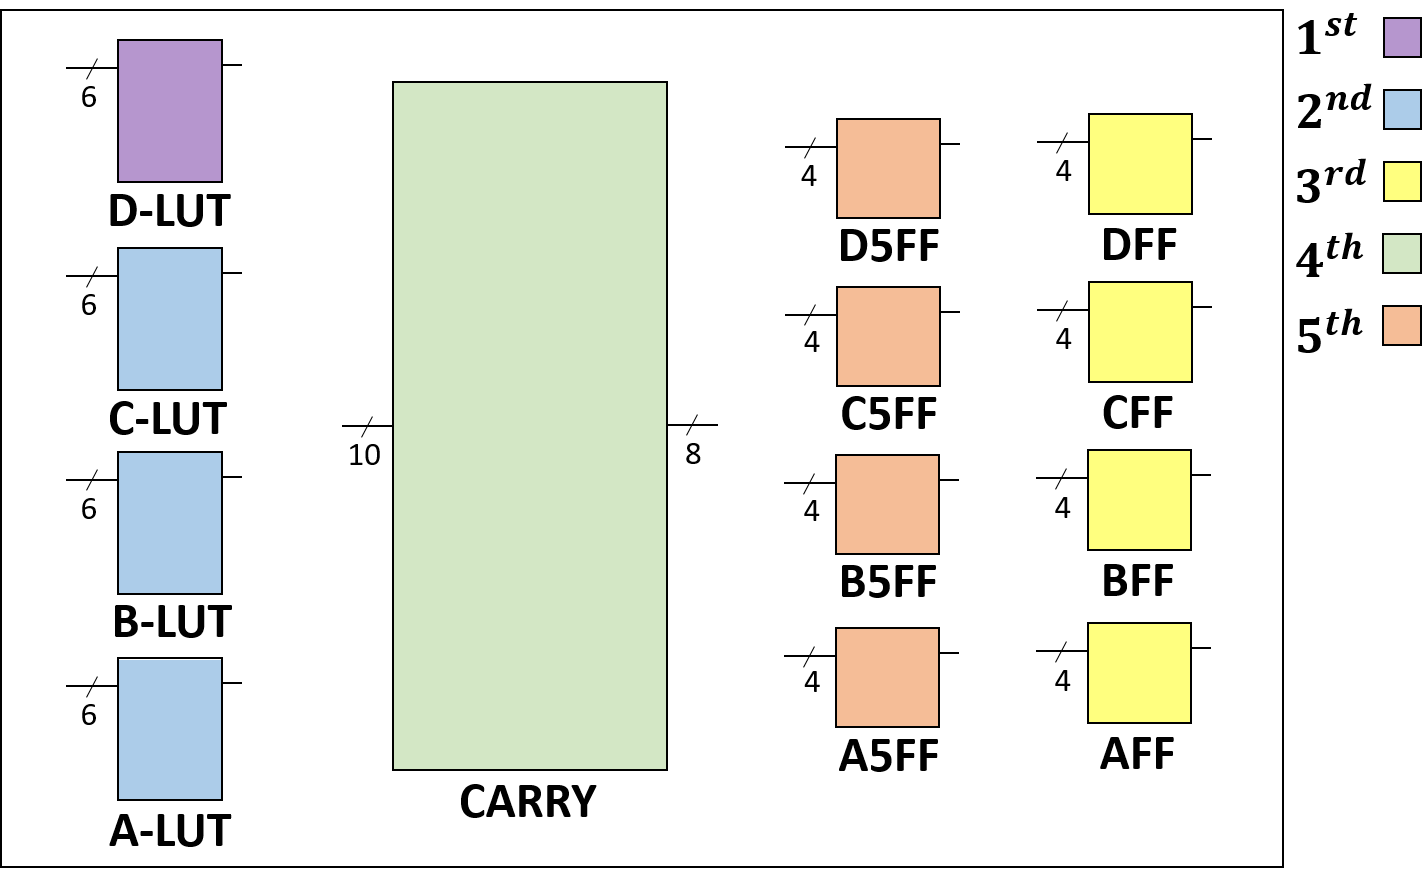
\includegraphics[width=.7\columnwidth]{slicePlacementOrder.png}
  \caption{Required placement order for Series7 SLICE sites. The figure shows a
  simplified representation of a SLICEL site.}
  \label{fig:slicePlacementOrder}
\end{figure}


For Series7 devices, experimentation has shown that the proper placement order
for groups of cells mapped to SLICE sites is as shown in
\autoref{fig:slicePlacementOrder}. The D6LUT needs to be placed first for
distributed memory cells. If the required placement order is not followed when
recreating a design, internal routing conflicts will occur that Vivado will be
unable to resolve. It is the responsibility of external tools to sort the cells
of a design in the proper order shown in \autoref{fig:slicePlacementOrder} when
creating the \textit{placement.rsc} file of a TCP.

It is important to note that the SLICE architecture of UltraScale
devices is significantly different than the Series7. Specifically, SLICE sites
in UltraScale have 8 LUTs (H-A), 16 FFs, and a CARRY8 instead of a CARRY4. In
initial testing, it appears that the placement order for UltraScale designs is
less strict. The only requirement is that the H6LUT (top-most LUT in the SLICE)
be placed first for distributed memory.

\subsubsection{Macro Placement} \label{sec:macroPlacement}

As described in Section~\ref{sec:macros} fully-flattened Vivado netlists may
include macro primitives. Section~\ref{sec:vdiImport} describes how macros
are exported from Vivado in RSCP files. Importing macro primitives
back into Vivado using TCP files, however, is a little more complicated. This
is because internal cells to a macro cannot be placed with XDC Tcl commands
(setting the property of an internal cell is an unauthorized operation in
Vivado). Therefore, external tools have two options when generating a TCP with
macros:

\begin{enumerate}
  \item Before creating the TCP, completely flatten the design netlist so that
  all macros are completely removed from the design.
  
  \item Support relatively placed macros (RPM), and output the placement
  information for just the RPM (not the internal cells) to the TCP. RPMs are
  macro cells that are assigned an anchor BEL placement location, and internal
  cells to the macro are placed \textit{relative} to the anchor.
\end{enumerate}

\noindent In general, the easier of the two solutions is to flatten the
design netlist completely, but either solution is valid with VDI. 

\subsubsection{LUT Routethroughs} \label{sec:routethroughReplace}

As described in Section~\ref{sec:routingRsc}, the \texttt{CONFIG.EQN} property on a
LUT BEL can be used to identity it as routethrough. On design export, all LUTs
in a design whose configuration equation matches that of a routethrough are
marked in the generated RSCP. It would stand to reason that when importing a
design back into Vivado, routethroughs could be recreated by setting the
corresponding \texttt{CONFIG.EQN} of the BEL. \texttt{CONFIG.EQN}, however, is
a \textbf{read-only} property, meaning the value can be queried but not
modified. Explicitly configuring a BEL's properties using the Tcl command
\texttt{[set\_property]} will throw an error in Vivado. These properties can
only be modified internally during the placement or routing stage of
implementation. Due to these limitations, it is currently not possible
to configure a BEL LUT as a routethrough in Vivado.

Therefore, it is the responsibility of external tools to replace all LUT
routethroughs in a design with a Xilinx \texttt{LUT1} cell before generating a
TCP. The general method for this is shown in \autoref{fig:routethroughReplace}.

\begin{figure}[h]
  \centering
  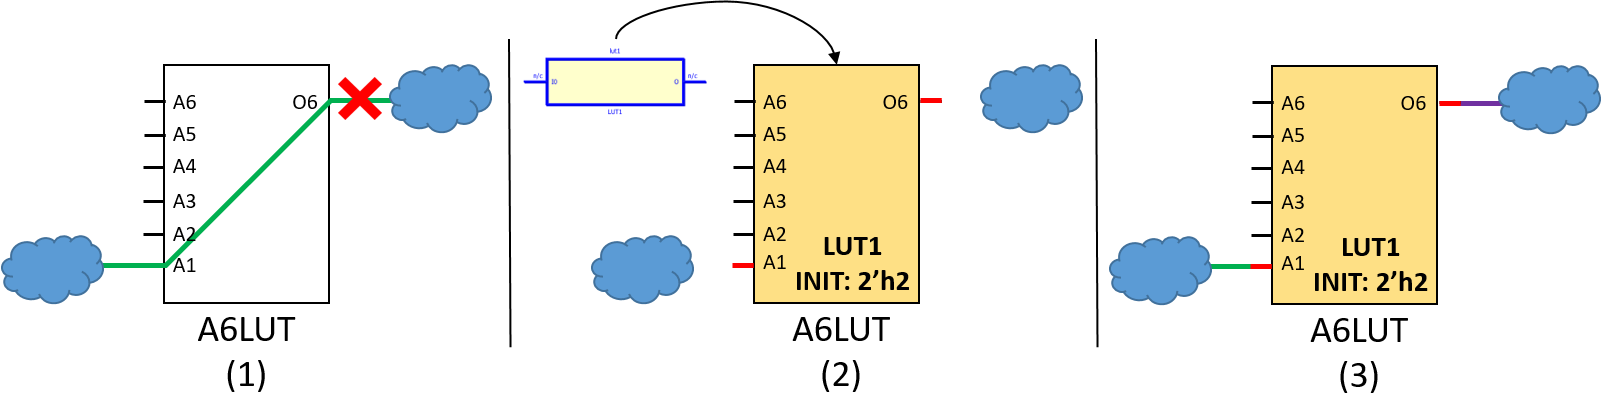
\includegraphics[width=\columnwidth]{routethroughReplace.png}
  \caption{Visualization for how to replace a LUT routethrough with a LUT1 Xilinx cell.}
  \label{fig:routethroughReplace}
\end{figure}

\noindent First, disconnect the routethrough net from all
downhill sink cell pins. Next, create a new \texttt{LUT1} Xilinx
library cell with a unique name and set the cell's \texttt{INIT} property to
``2'h2'' (this configures the cell to be a passthrough LUT). Place the cell
onto the BEL that was formerly being used as a routethrough, and map the
\texttt{I0} input pin of the cell to the corresponding routethrough BEL pin
(\texttt{A1} in the case of the example). Rewire the netlist and connect
the original routethrough net to pin \texttt{I0} of the new cell. The final
step is to create a new net with a unique name, and connect it to the
output pin of the new cell and the downhill logic disconnected earlier. Once
this is complete, the netlist now explicitly represents the routethrough, and
valid TCPs can be generated.

\subsubsection {Routing Differential Pairs}
Xilinx devices support differential input signals for design input. An example
differential pairing is shown in \autoref{fig:diffInput}. The net highlighted in
white connects the two differential signals together for Xilinx to resolve to a
single value. As can be seen, the physical route of the net is very simple, with
only a single PIP connection. As a TCP is being imported, however, Vivado is
unable to correctly process the \texttt{ROUTE} strings for these nets.
Specifically, when the \texttt{ROUTE} string for a differential net is
specified, the following error message is given: ``\texttt{ERROR: [Designutils
20-949] No driver found on net netname}''. 

The function \texttt{[tincr::read\_tcp]} provides a workaround by first routing
all other nets in the design. Once all other nets have been routed, the Tcl code
shown in \autoref{lst:diffNet} is run. The differential nets are identified
using the Tcl command on line 1, and each net is individually routed by Vivado's
router. Since there is only one possible route between the source and the sink
pin, the differential nets will be routed correctly. The downfall to this
approach is that it can take up to 1 minute to finish routing all differential
nets. It is important to note that this is only an issue for Series7 devices,
and is not needed for UltraScale.

\begin{lstlisting}[xleftmargin=1.5em, framexleftmargin=1.5em, keywordstyle=,
stringstyle=, caption= Tcl script to route differential nets in Vivado, label=lst:diffNet]
set diff [get_nets -of [get_ports] -filter {ROUTE_STATUS != INTRASITE} -quiet]

if {[llength $diff] > 0 } {
	route_design -quiet -nets $diff
}
\end{lstlisting}

\begin{figure}[t!]
  \centering
  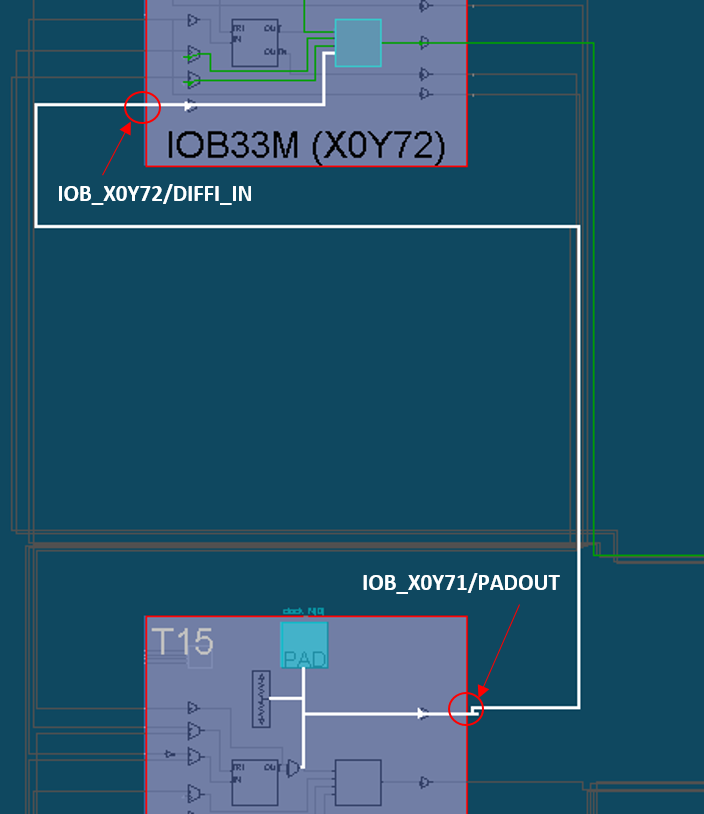
\includegraphics[width=.6\columnwidth]{diffInput.png}
  \caption{Differential Pair Net}
  \label{fig:diffInput}
\end{figure}

\subsection{Why Two Design Checkpoint Formats?} \label{sec:twoFormats}
So far this chapter has described in great detail RSCPs, TCPs, and the
associated Vivado Tcl challenges with both. There is, however, one more
question to consider: ``Why can't a single design format be used for external
tools \textit{and} Vivado''? Here are four reasons why both RSCPs and TCPs are
required with VDI:

\begin{enumerate}
  \item Some Vivado design representations cannot be used with
  external tools. This is best shown with Vivado \texttt{ROUTE} strings, which
  are used to represent the physical route of a net. Due to the ambiguities of
  \texttt{ROUTE} strings as described in Section~\ref{sec:routeStrings}, they are
  not suitable for design export (PIPs must be used instead). However,
  \texttt{ROUTE} strings are required when importing a design back into Vivado
  (Section~\ref{sec:routingXdc}). This indicates that a different format is needed
  for exporting and importing the physical structure of a net.
     
  \item When an external design is imported into Vivado, some physical
  implementation details of the design are automatically configured. 
  For example, site PIPs, static source LUTs, and intrasite nets are all
  configured during placement import based on how the cells of a design are
  placed. These design aspects do not need to be explicitly represented in a
  TCP. External tools don't have the luxury of automatic configuration, and so
  these details do need to be explicitly represented in a RSCP. Otherwise, a
  design could only be partially represented.
    
  \item RSCPs and TCPs are designed for different purposes. TCPs are
  designed to import a design into Vivado as \textbf{quickly as possible}. The
  XDC format allows for this due to the dedicated Tcl command
  \texttt{[read\_xdc]}. RSCPs are designed to be \textbf{easily parse-able}, and
  use a simple token-based scheme with whitespace separated values.
  
  \item Vivado offers a native checkpoint format (DCP) that can be used to save
  and restore the progress of an implemented design. Due to this available
  checkpoint format, there is no reason to support importing RSCPs directly back
  into Vivado. Users that want this capability can use DCPs, allowing RSCP
  checkpoints to be more customized.
  
\end{enumerate}